\section{Architecture Integration}

\subsection{Model Support}

\begin{table}[H]
\centering
\small
\begin{tabular}{lllll}
\toprule
\textbf{Model} & \textbf{Attention} & \textbf{Nested?} & \textbf{RoPE?} & \textbf{GQA?} \\
\midrule
DistilBERT & \texttt{layer[i].attention} & No & No & No \\
RoBERTa & \texttt{layer[i].attention.self} & Yes & No & No \\
GPT-2 & \texttt{h[i].attn} & No & No & No \\
Qwen3.5 & \texttt{layers[i].self\_attn} & No & Yes & Yes \\
\bottomrule
\end{tabular}
\end{table}

\subsection{Weight Extraction}

The \texttt{copy\_weights} procedure handles four patterns:

\subsubsection{GPT-2 Conv1D}

\begin{lstlisting}
c\_w = c\_attn.weight.t()
q\_w, k\_w, v\_w = c\_w.chunk(3, dim=0)
o\_w = c\_proj.weight.t()
\end{lstlisting}

\subsubsection{RoBERTa Nested}

\begin{lstlisting}
q\_w = src.self.query.weight
k\_w = src.self.key.weight
v\_w = src.self.value.weight
o\_w = src.output.dense.weight
\end{lstlisting}

\subsubsection{Flat Modules}

\begin{lstlisting}
q\_w = src.q\_lin.weight  # or q\_proj or query
\end{lstlisting}

\subsubsection{UniversalAdapter}

Fallback if none match.

\subsection{Handling of the RFF Projection}

The RFF matrix $\Omega$ has \textbf{no pretrained equivalent} -- it is initialized 
randomly. This is intentional: random features are theoretically justified 
by Bochner's theorem, and the adaptive gate can down-weight the linear 
stream if $\Omega$ is not useful.

\subsection{Gate Initialization}

The gate is a \texttt{Linear(dim, H)} module with:

\begin{itemize}
\item Weight zero-initialized.
\item Bias = 5.0.

\end{itemize}
This makes $\sigma(b_g) \approx 0.993$, favoring the dense stream.

\subsection{Nested Encoder Bypass}

For RoBERTa, \texttt{is\_nested\_encoder = True}, so we \textbf{do not} apply \texttt{out\_proj}. 
The outer \texttt{attention.output.dense} handles the projection.

\subsection{GQA Support}

For GQA models (Qwen), we expand K, V via \texttt{repeat\_kv} before both streams.

\subsection{RoPE Support}

Partial-coordinate RoPE:

\begin{lstlisting}
if rotary\_dim \textless{} head\_dim:
    q\_rot, q\_pass = q[..., :rotary\_dim], q[..., rotary\_dim:]
    q = torch.cat([q\_rot * cos + rot(q\_rot) * sin, q\_pass], dim=-1)
\end{lstlisting}

\subsection{Causality}

For decoders, we apply:

\begin{enumerate}
\item \textbf{Dense stream:} causal mask on scores.
\item \textbf{Linear stream:} cumsum over sequence.

\end{enumerate}
Both are strictly causal.

\subsection{Injection Algorithm}

\textbf{Algorithm 2:} Inject CHELA-SLAY into a model
\begin{lstlisting}
Input:  model M, config c
Output: M with attention replaced

1: for each layer with attention:
2:     src $\leftarrow$ extract\_attention(layer)
3:     if src is None: continue
4:     try:
5:         new $\leftarrow$ ChelaSlayAttention(c, pretrained\_attn=src)
6:         replace(layer, new)
7:     except Exception:
8:         raise RuntimeError("copy\_weights failed")
9: return M
\end{lstlisting}

\subsection{Failure Handling}

The injection raises \texttt{RuntimeError} on any failure. This is strict but 
appropriate because the hybrid attention is complex.

\subsection{Registry}

\begin{lstlisting}
@ATTENTION\_REGISTRY.register("chela\_slay")
@ATTENTION\_REGISTRY.register("chela\_slay\_attention")
class ChelaSlayAttention(BaseAttention):
    ...
\end{lstlisting}



\begin{figure}[H]
\centering
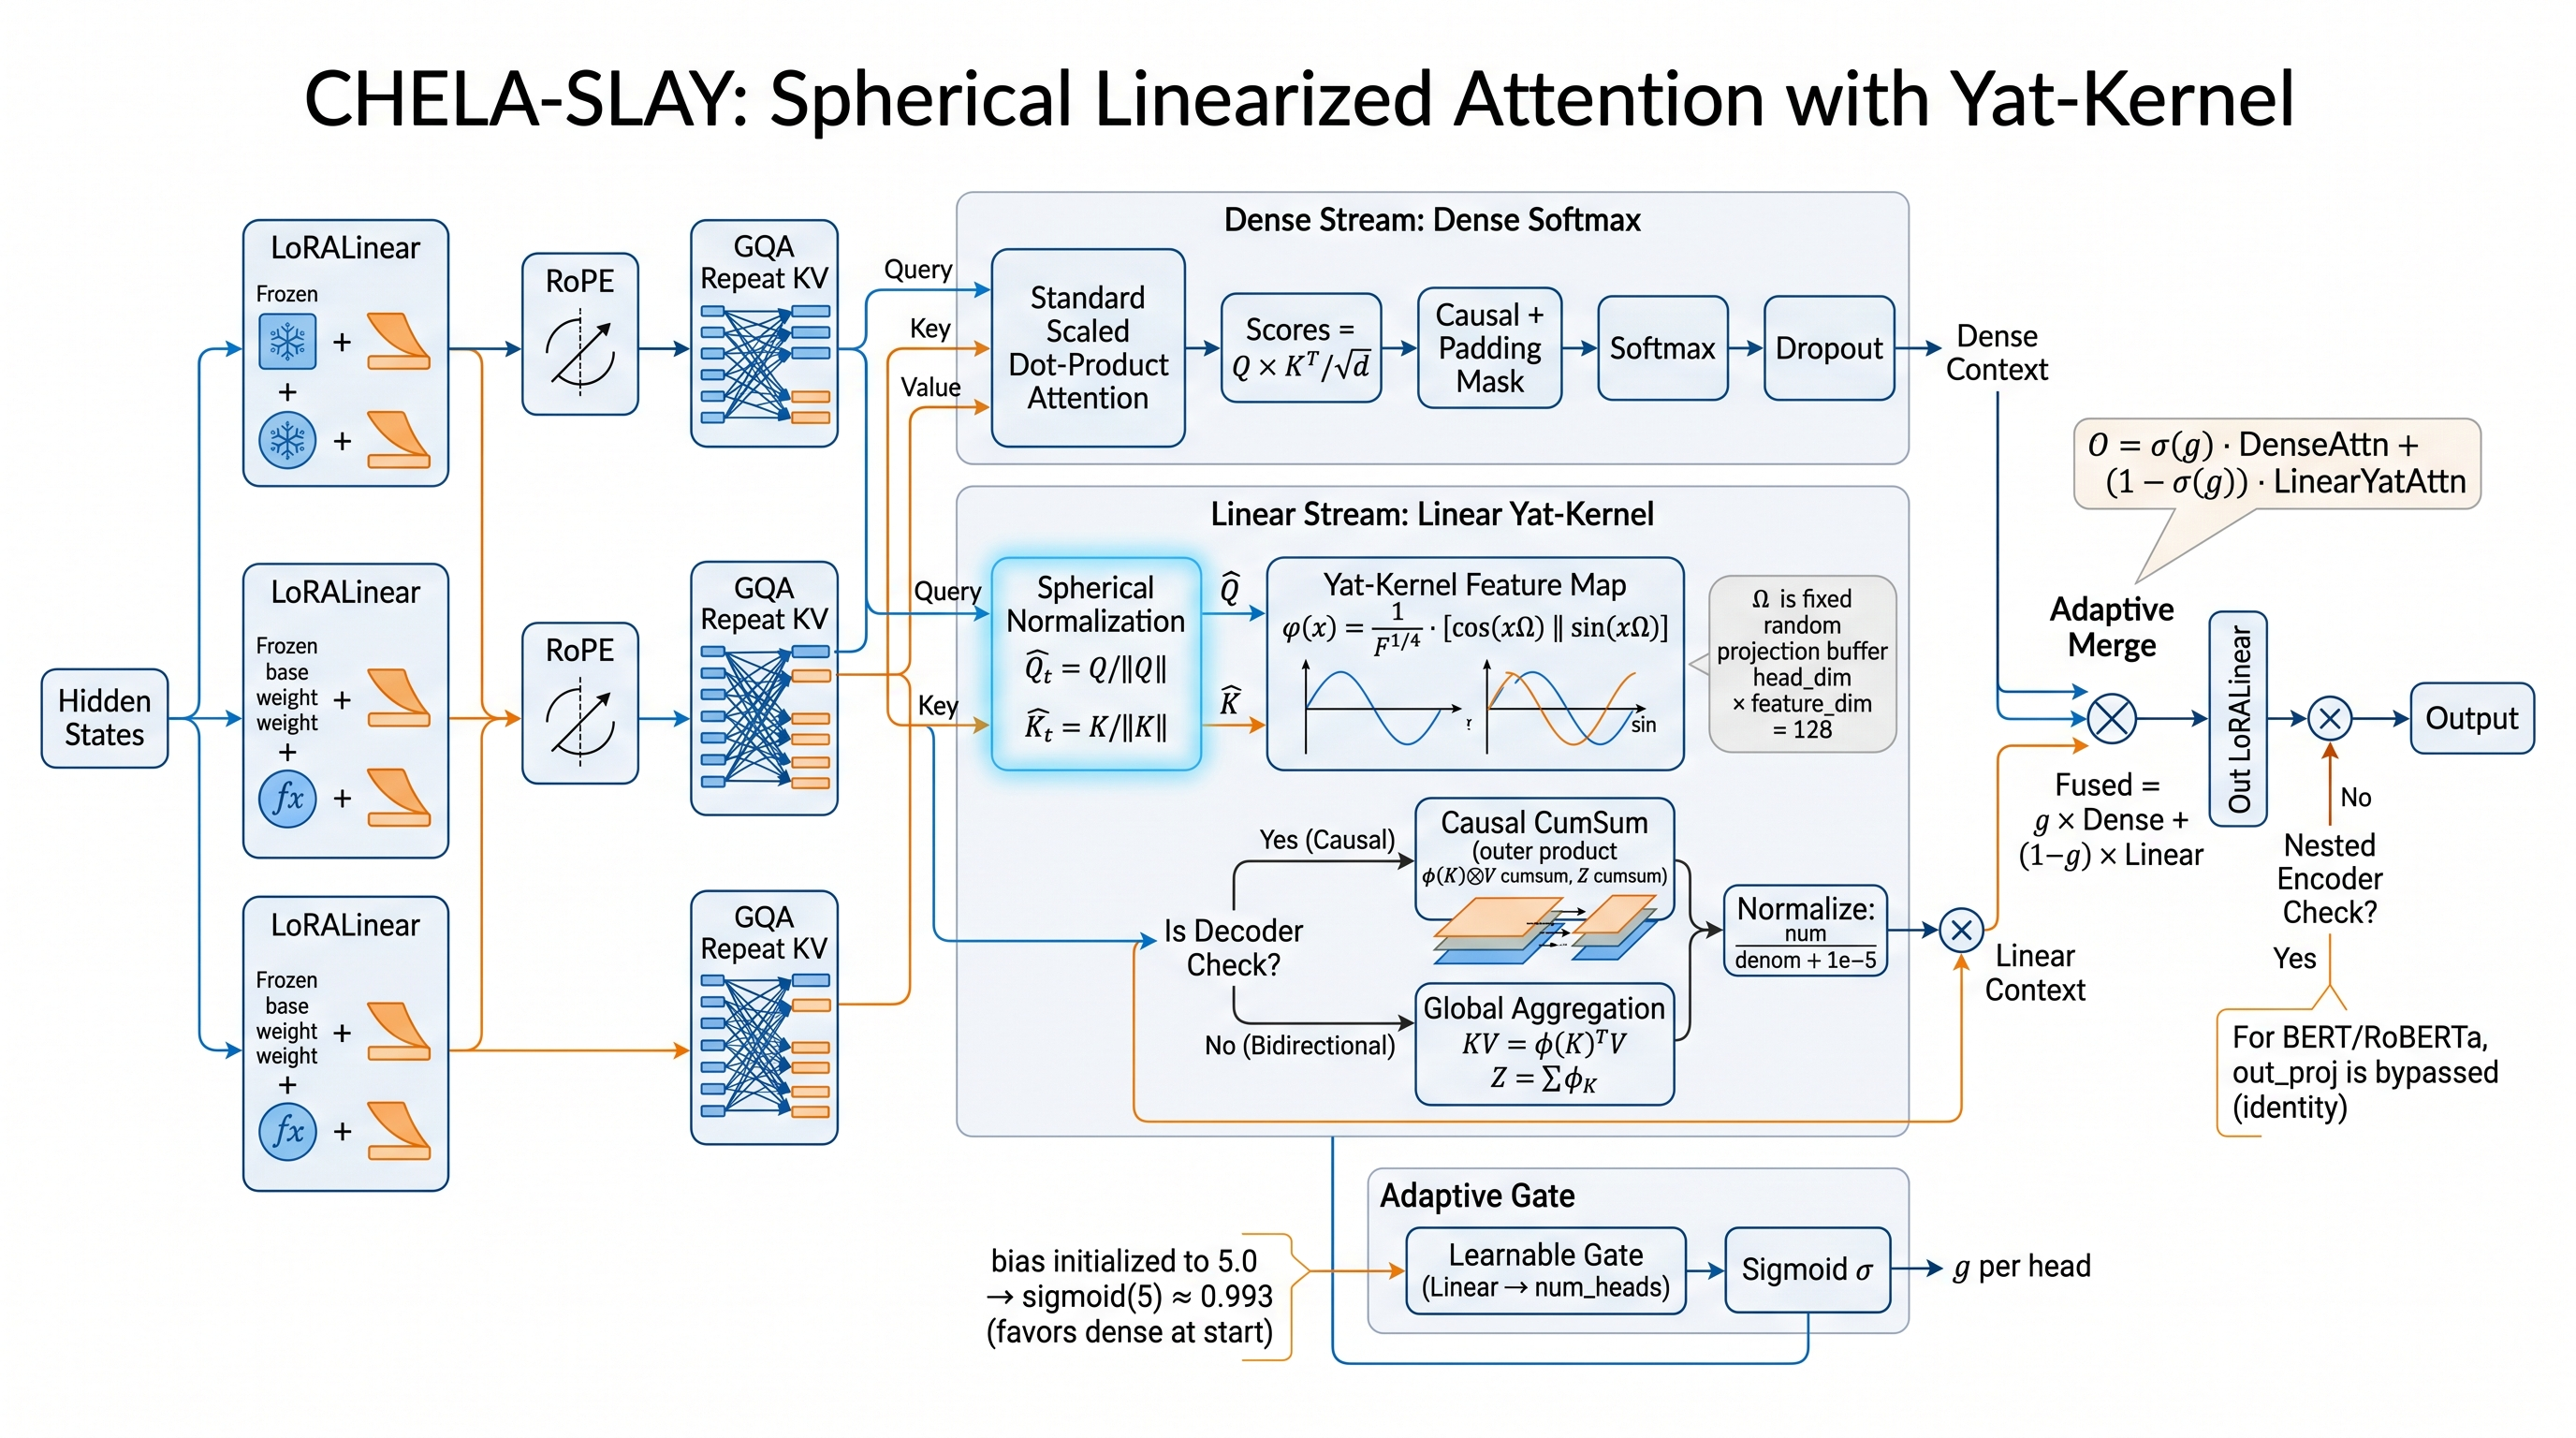
\includegraphics[width=\linewidth]{figures/architecture.jpeg}
\caption{High-level architectural diagram of chela\_slay.}
\label{fig:arch_chela-slay}
\end{figure}

